\documentclass[11pt,]{article}
\usepackage[left=1in,top=1in,right=1in,bottom=1in]{geometry}
\newcommand*{\authorfont}{\fontfamily{phv}\selectfont}
\usepackage[]{mathpazo}


  \usepackage[T1]{fontenc}
  \usepackage[utf8]{inputenc}



\usepackage{abstract}
\renewcommand{\abstractname}{}    % clear the title
\renewcommand{\absnamepos}{empty} % originally center

\renewenvironment{abstract}
 {{%
    \setlength{\leftmargin}{0mm}
    \setlength{\rightmargin}{\leftmargin}%
  }%
  \relax}
 {\endlist}

\makeatletter
\def\@maketitle{%
  \newpage
%  \null
%  \vskip 2em%
%  \begin{center}%
  \let \footnote \thanks
    {\fontsize{18}{20}\selectfont\raggedright  \setlength{\parindent}{0pt} \@title \par}%
}
%\fi
\makeatother




\setcounter{secnumdepth}{3}

\usepackage{longtable,booktabs}

\usepackage{graphicx,grffile}
\makeatletter
\def\maxwidth{\ifdim\Gin@nat@width>\linewidth\linewidth\else\Gin@nat@width\fi}
\def\maxheight{\ifdim\Gin@nat@height>\textheight\textheight\else\Gin@nat@height\fi}
\makeatother
% Scale images if necessary, so that they will not overflow the page
% margins by default, and it is still possible to overwrite the defaults
% using explicit options in \includegraphics[width, height, ...]{}
\setkeys{Gin}{width=\maxwidth,height=\maxheight,keepaspectratio}

\title{Título\\[2\baselineskip]  }



\author{\Large Melany Karina Ogando Matos\vspace{0.05in} \newline\normalsize\emph{Estudiante, Universidad Autónoma de Santo Domingo (UASD)}  }


\date{}

\usepackage{titlesec}

\titleformat*{\section}{\normalsize\bfseries}
\titleformat*{\subsection}{\normalsize\itshape}
\titleformat*{\subsubsection}{\normalsize\itshape}
\titleformat*{\paragraph}{\normalsize\itshape}
\titleformat*{\subparagraph}{\normalsize\itshape}

\titlespacing{\section}
{0pt}{36pt}{0pt}
\titlespacing{\subsection}
{0pt}{36pt}{0pt}
\titlespacing{\subsubsection}
{0pt}{36pt}{0pt}





\newtheorem{hypothesis}{Hypothesis}
\usepackage{setspace}

\makeatletter
\@ifpackageloaded{hyperref}{}{%
\ifxetex
  \PassOptionsToPackage{hyphens}{url}\usepackage[setpagesize=false, % page size defined by xetex
              unicode=false, % unicode breaks when used with xetex
              xetex]{hyperref}
\else
  \PassOptionsToPackage{hyphens}{url}\usepackage[unicode=true]{hyperref}
\fi
}

\@ifpackageloaded{color}{
    \PassOptionsToPackage{usenames,dvipsnames}{color}
}{%
    \usepackage[usenames,dvipsnames]{color}
}
\makeatother
\hypersetup{breaklinks=true,
            bookmarks=true,
            pdfauthor={Melany Karina Ogando Matos (Estudiante, Universidad Autónoma de Santo Domingo (UASD))},
             pdfkeywords = {palabra clave 1, palabra clave 2},  
            pdftitle={Título\\[2\baselineskip]},
            colorlinks=true,
            citecolor=blue,
            urlcolor=blue,
            linkcolor=magenta,
            pdfborder={0 0 0}}
\urlstyle{same}  % don't use monospace font for urls

% set default figure placement to htbp
\makeatletter
\def\fps@figure{htbp}
\makeatother

\usepackage{pdflscape} \newcommand{\blandscape}{\begin{landscape}}
\newcommand{\elandscape}{\end{landscape}} \usepackage{float}
\floatplacement{figure}{H}
\newcommand{\beginsupplement}{ \setcounter{table}{0} \renewcommand{\thetable}{S\arabic{table}} \setcounter{figure}{0} \renewcommand{\thefigure}{S\arabic{figure}} }


% add tightlist ----------
\providecommand{\tightlist}{%
\setlength{\itemsep}{0pt}\setlength{\parskip}{0pt}}

\begin{document}
	
% \pagenumbering{arabic}% resets `page` counter to 1 
%
% \maketitle

{% \usefont{T1}{pnc}{m}{n}
\setlength{\parindent}{0pt}
\thispagestyle{plain}
{\fontsize{18}{20}\selectfont\raggedright 
\maketitle  % title \par  

}

{
   \vskip 13.5pt\relax \normalsize\fontsize{11}{12} 
\textbf{\authorfont Melany Karina Ogando Matos} \hskip 15pt \emph{\small Estudiante, Universidad Autónoma de Santo Domingo (UASD)}   

}

}








\begin{abstract}

    \hbox{\vrule height .2pt width 39.14pc}

    \vskip 8.5pt % \small 

\noindent Resumen del manuscrito


\vskip 8.5pt \noindent \emph{Keywords}: palabra clave 1, palabra clave 2 \par

    \hbox{\vrule height .2pt width 39.14pc}



\end{abstract}


\vskip 6.5pt


\noindent  \section{Introducción}\label{introducciuxf3n}

Ahora estoy insertando bibliografia, si lo quiero entre parentesis
(Hubbell et al., 1999), y si lo quiero parte del texto Hubbell et al.
(1999).

Para citar dos autores (Hubbell et al., 1999, Sun, Rosin, Martin, \&
Langbein (2007))

\section{Metodología}\label{metodologuxeda}

Aqui va la metodologia.

\section{Resultados}\label{resultados}

La familia Chrysobalanaceae esta compuesta por 4 especies dispuestas en
dons generos: Hirtella american y triandra, y Licania hypoleuca y
platypus. La especie mas abundante es Hirtella triandra con 4,408; le
sigue Licania platypus con 251, Licania hypoeluca con 141, e Hirtella
americana con 21. El numero total de individuos es 4,821.

Los lugares 34 y 38 revisar. (Ver figura \ref
{cuadroabun})

Ahora vamos a insertar imagen:

\begin{figure}
\centering
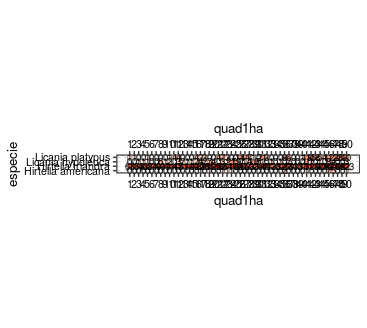
\includegraphics[width=0.80000\textwidth]{Abun_por_cuadro.png}
\caption{Abundancia de mi familia por cuadrante\label{cuadroabun}}
\end{figure}

Vamos a editar la imagen ahora: \ref{fig:abunsp}

\begin{figure}
\centering
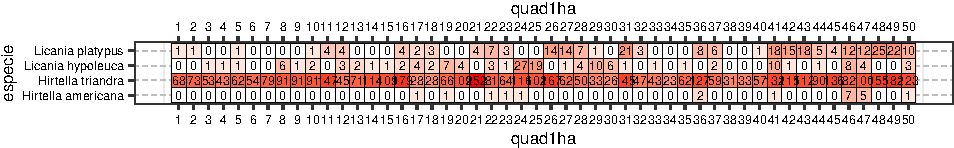
\includegraphics{manuscrito_files/figure-latex/unnamed-chunk-2-1.pdf}
\caption{\label{fig:abunsp}Abundancia de especies por cuadros}
\end{figure}

Y ahora una tabla:

\begin{longtable}[]{@{}ll@{}}
\toprule
Especie & Abundancia\tabularnewline
\midrule
\endhead
1 & 10\tabularnewline
2 & 20\tabularnewline
3 & 30\tabularnewline
4 & 40\tabularnewline
\bottomrule
\end{longtable}

Insertar tabla con knitr: Aqui esta la referencia \ref{tab:tababun}

\begin{longtable}[]{@{}lr@{}}
\caption{\label{tab:tababun}Abundancia de especies de la familia
Chrysobalaneceae}\tabularnewline
\toprule
Latin & n\tabularnewline
\midrule
\endfirsthead
\toprule
Latin & n\tabularnewline
\midrule
\endhead
Hirtella triandra & 4408\tabularnewline
Licania platypus & 251\tabularnewline
Licania hypoleuca & 141\tabularnewline
Hirtella americana & 21\tabularnewline
\bottomrule
\end{longtable}

\section{Discusión}\label{discusiuxf3n}

\section{Agradecimientos}\label{agradecimientos}

\section{Información de soporte}\label{informaciuxf3n-de-soporte}

\section{\texorpdfstring{\emph{Script}
reproducible}{Script reproducible}}\label{script-reproducible}

\section*{Referencias}\label{referencias}
\addcontentsline{toc}{section}{Referencias}

\hypertarget{refs}{}
\hypertarget{ref-hubbell1999light}{}
Hubbell, S. P., Foster, R. B., O'Brien, S. T., Harms, K. E., Condit, R.,
Wechsler, B., \ldots{} De Lao, S. L. (1999). Light-gap disturbances,
recruitment limitation, and tree diversity in a neotropical forest.
\emph{Science}, \emph{283}(5401), 554--557.

\hypertarget{ref-sun2007fast}{}
Sun, X., Rosin, P., Martin, R., \& Langbein, F. (2007). Fast and
effective feature-preserving mesh denoising. \emph{IEEE Transactions on
Visualization \& Computer Graphics}, (5), 925--938.




\newpage
\singlespacing 
\end{document}
